\documentclass[a4paper,10pt]{article}
\usepackage[utf8x]{inputenc}

\usepackage{verse}
\usepackage[slovene]{babel}
\usepackage{graphicx}
\usepackage{hyperref}
\usepackage{amsmath}
\usepackage{amsfonts}
\usepackage{comment}
\usepackage{subfigure}

\usepackage[table]{xcolor}

\newcommand{\slika}[2]{
\begin{figure}[h]
 \input{#1}
  \caption{#2}
  \label{fig:#1}
\end{figure}
}

\newcommand{\dd}{\,\mathrm{d}}

\title{Generatorji slu\v cajnih \v stevil}
\author{Miha \v Can\v cula}

\begin{document}
 \maketitle

\begin{abstract}
 The generation of random numbers is too important to be left to chance.
     -- Robert R. Coveyou, \textit{Oak Ridge National Laboratory}
\.\\
\begin{figure}[h!]
\centering
  \subfigure{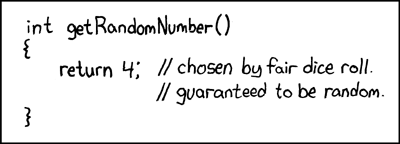
\includegraphics[width=250pt]{random-xkcd}}\\
  \subfigure{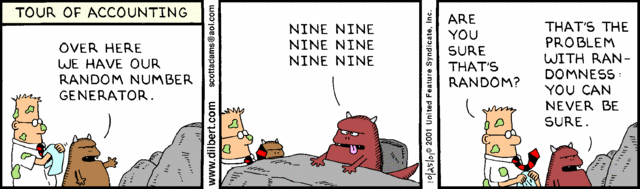
\includegraphics[width=300pt]{random-dilbert}}
\end{figure}
\end{abstract}

\section{Enakomerne porazdelitve}

Najenostavnej"sa je bila primerjava med generatorji, ki vrnejo naklju"cna "stevila, ki so enakomerno razporejena po nekem intervalu. Tak"snih generatorjev je tudi najve"c, zato sem jih lahko primerjal. Za vsakega sem izra"cunal porazdelitev verjetnosti z razdelitvijo v $B$ predal"ckov, nato pa na ti porazdelitvi izvajal statisti"cne teste. Uporabil sem naslednje generatorje:

\begin{enumerate}
 \item Funkcija \texttt{rand()} iz standardne knji"znice jezika \texttt{C}
 \item Linuxova datoteka \texttt{/dev/urandom}
 \item Kalkulatorski generator, opisan v navodilih
 \item ``Mersennov vrtinec'', implementiran v \texttt{GSL} 
\end{enumerate}

Poleg teh generatorjev sem za primerjavo vklju"cil "se dva izvora naklju"cnih "stevil, ki "stevil ne generirata s "stevilskim algoritmom, ampak jih izra"cunata te"zko predvidljivih dogodkov. V nasprotju z generatorji na ta na"cin ne moremo dobiti poljubnega "stevila naklju"cnih "stevil, zato sem velikost vzorca omejih na 4096 "stevil, kjer ima vsako "stevilo 32 bitov.

\begin{enumerate}
 \item Linuxova datoteka \texttt{/dev/random}, ki naklju"cnost dobi iz dogodkov v ra"cunalniku, na primer s premikanjem mi"ske
 \item Spletna stran \texttt{random.org}, ki naklju"cnost dobi iz meritev atmosferskega "suma
\end{enumerate}

"Zal se je izkazalo, da je branje iz \texttt{/dev/random} prepo"casno za kakr"snekoli statisti"cne teste, saj sem le po divjem mahanju z mi"sko uspel dobiti 100 naklju"cnih "stevil. To je dovolj za generiranje naklju"cnih gesel in "sifrirnih klju"cev, ne pa za statistiko, zato sem ta generator izpustil iz nadaljnjih ra"cunov. 

Za vse statisti"cne teste $\chi^2$ sem v tabelo vpisal verjetnosti, poleg tega pa sem dodal "se pri"cakovane vrednosti za idealen generator naklju"cnih "stevil. Testu Kolmogorov-Smirnova sem opravil brez predal"ckanja, tako da sem generirana "stevila najprej uredil, nato pa njihovo kumulativno porazdelitev primerjal s pri"cakovano. Vpisal sem dobljeno vrednosti statistike $D$, ki bi pri stopnji tveganja 5\% morala biti ni"zja od 1,36. Pri enodimenzionalnih testih sem podatke razdelil v $\sqrt{N}$ predal"ckov, pri dvodimenzionalnih pa v $\sqrt[3]{N} \times \sqrt[3]{N}$ predal"ckov. Z rde"co barve sem ozna"cil vrednosti, ki bi jih lahko zavrgli z manj kot 5\% tveganjem. 

\begin{table}[h]
 \centering
  \begin{tabular}{|c|c|c|c|c|c|c|c|c|c|c|}
  \hline
  Test & \multicolumn{3}{|c|}{1D $\chi^2$} & \multicolumn{3}{|c|}{2D $\chi^2$} & \multicolumn{3}{|c|}{$D\sqrt{N}$} & "Cas [s]\\
  \hline
  $N$ & $2^{12}$ & $2^{18}$ & $2^{24}$ & $2^{12}$ & $2^{18}$ & $2^{24}$ & $2^{12}$ & $2^{18}$ & $2^{24}$ & $2^{28}$ \\
  \hline
  \texttt{rand()} & 35\% & 32\% & 34\% & 65\% & 57\% & 29\% & 0,52 & 1,22 & 0,59 & 3.3 \\
  \texttt{/dev/urandom} & 54\% & 61 \% & 29\% & 21\% & 53\% & 84\% & 0,74 & 1,17 & 0,47 & 110 \\
  Kalkulatorski & 74\% & \cellcolor{red} 98\% & \cellcolor{red} 0\% & 70\% & \cellcolor{red} 4\% & \cellcolor{red} 0\% & 0,49 & 0,69 & \cellcolor{red} 15,2 & 36 \\
  Mersenne & 17\% & 71\% & 63\% & \cellcolor{red} 0,5\% & 50\% & 62\% & 0,90 & 1,07 & 0,63 & 2.9 \\
\hline
  \texttt{random.org} & 28\% & & & 49\% & & & 0,90 & & & \\
\hline
  Idealno & \multicolumn{3}{|c|}{50\%} & \multicolumn{3}{|c|}{50\%} & \multicolumn{3}{|c|}{1} & \\
\hline
   
  \end{tabular}
\caption{Statisti"cni testi enakomernosti naklju"cnih "stevil}
\end{table}

Pri obeh testih $\chi^2$ si "zelimo verjetnost "cim bli"zje 50\%. Premajhna vrednosti (npr. manj kot 5\%) pomeni, da lahko generator zavr"zemo z majhno stopnjo tveganja, saj "stevila niso porazdeljena dovolj enakomerno. Podobno pa prevelika vrednost (npr. ve"c kot 95\%) pomeni, da je porazdelitev preve"c enakomerna, saj so odstopanja manj"sa od pri"cakovane statisti"cne napake. Oboje namre"c pomeni, da "stevila niso naklju"cna. 

Iz podatkov lahko zaklju"cimo, da je izmed preizku"sanih generatorjev najbolj"si Mersennov vrtinec. Izka"ze se predvsem, "ce moramo generirati veliko naklju"cnih "stevil, tako z dobrimi rezultati testov kot tudi s hitrostjo. Pri manj"sih vzorcih je verjetno enostavneje izbrati vgrajeni generator, ki se pona"sa s podobno hitrostjo, in celo z bolj"sim $\chi^2$ za dovolj majhne $N$. Kalkulatorski generator je v vseh primerih najslab"si. 


\section{Smeri v prostoru}

Za generacijo naklju"cnih meri v prostoru najprej potrebujemo generator enakomernih naklju"cnih "stevil. V ta namen sem uporabil kar najbolj"si generator iz prve naloge, to je bil Mersennov vrtinec. Knji"znica \texttt{GSL} ima vgrajeno rutino, ki s pomo"cjo enakomernega generatorja vrne naklju"cen enotski vektor v treh dimenzijah. Kljub temu pa sem za primerjavo "se sam napisal tak"sen generator. Za primer brez sevanja je algoritem enostaven, saj vemo da mora biti porazdelitev verjetnosti enakomerna po spremenljivkah $\varphi$ in $\cos\vartheta$. "Ce sta $r_1$ in $r_2$ dve naklju"cni "stevili med 0 in 1, lahko prostorski kot zapi"semo kot

\begin{align}
 \varphi &= 2\pi r_1 \label{eq:ran-smer-phi}\\
 \vartheta &= \arccos (2r_2-1) \label{eq:ran-smer-theta}
\end{align}

Paziti moramo, da je $r_1 \in [0,1)$ in $r_2 \in [0,1]$, saj kota $\varphi = 0$ in $\varphi = 2\pi$ predstavljata isto koordinato na krogli, medtem ko sta $\vartheta=0$ in $\vartheta=\pi$ razli"cni to"cki. Zaradi omejene natan"cnosti strojnega ra"cunanja sem to moral upo"stevati pri generiranju "stevil. 

Pri dipolnem sevanju je porazdelitev verjetnosti po kotu $\vartheta$ bolj zapletena. 

\begin{align}
 \frac{\partial p}{\partial \vartheta} & \propto \sin^3\vartheta \\
  \dd p &= C \sin^3 \vartheta \dd \vartheta = C(1-\cos^2\vartheta) \dd (\cos\vartheta) \\
&= C \dd\left( \cos\vartheta - \frac{\cos\vartheta^3}{3} \right)
\end{align}

"Ce upostevamo, da je $r_2$ enakomerno razporejen, dobimo ena"cbo za $\vartheta$. 

\begin{align}
\frac{\cos^3\vartheta}{3} - \cos\vartheta + Ar_2 + B = 0
\end{align}

Da izrazimo $\cos\vartheta$ s pomo"cjo $r_2$ bomo morali re"siti polinom tretje stopnje. Ena"cba mora vedno imeti eno re"sitev za $\cos\vartheta$ na intervalu $[-1,1]$. Konstanti $A$ in $B$ torej dolo"cimo tako, da bo preslikava med $\cos\vartheta\in[-1,1]$ in $r_2\in[0,1]$ bijektivna. To do"sezemo, "ce je 

\begin{align}
\frac{\cos^3\vartheta}{3} - \cos\vartheta + \frac{2}{3}(2r_2 -1) = 0
\end{align}

V tem primeru ima polinom vedno tri realne korene, od katerih je srednji med $-1$ in $1$. 

\subsection{Krogelne funkcije}

Vrednosti za $\vartheta$ in $\varphi$ nisem razdelil v histogram, ampak sem izra"cunal pri"cakovane vrednosti nekaterih osnovnih momentov. Ra"cunal sem povprecji $\varphi$ in $\cos\theta$, povpre"cen kvadrat $\cos^2\theta$, poleg tega pa se krogelno funkcijo $Y_1^1 = \cos\varphi \cos\theta$, ki preverja korelacijo med obema spremenljivkama. Vse ra"cune sem izvajal z $N=2^{24}$ "stevili. Rezultati so v tabeli \ref{tab:smer}. 

\begin{table}[h]
\centering
\begin{tabular}{|c|c|c|c|c|}
 \hline
  Generator & $\langle \cos\vartheta \rangle$ & $\langle \varphi \rangle$ & $\langle \cos^2\vartheta \rangle$ & $\langle Y_1^1 \rangle$ \\
\hline
  Naklju"cna smer (\texttt{GSL}) & $-3,88 \cdot 10^{-5}$ & $14,0 \cdot 10^{-5}$ & 0.333326 & $5.58 \cdot 10^{-7}$ \\
  Naklju"cna smer (jaz) & $5,96 \cdot 10^{-5}$ & $-25,9 \cdot 10^{-5}$ & 0.333356 & $4,86 \cdot 10^{-5}$\\
\hline
  Pri"cakovano & 0 & 0 & 1/3 & 0 \\
\hline
\end{tabular}
\caption{Primerjava osnovnih momentov za obe implementaciji naklju"cne smeri v prostoru. }
\label{tab:smer}
\end{table}

Vidimo, da je moja implementacija generatorja naklju"cnih smeri, ki sledi ena"cbama (\ref{eq:ran-smer-phi}) in (\ref{eq:ran-smer-theta}), slab"sa od algoritma v \texttt{GSL}. Odstopanje od pri"cakovanega povpre"cja je bilo ve"cje v vseh treh kriterijih, kjer upo"stevamo le eno spremenljivko. Po drugi strani pa je korelacija med $\varphi$ in $\vartheta$ manj"sa, kar lahko razlo"zimo s tem, da v zgornjih ena"cbah ni povezave med $\vartheta$ in $\varphi$. 

\begin{table}[h]
\centering
\begin{tabular}{|c|c|c|c|c|}
 \hline
  Generator & $\langle \cos\vartheta \rangle$ & $\langle \varphi \rangle$ & $\langle \cos^2\vartheta \rangle$ & $\langle Y_1^1 \rangle$ \\
\hline
  Dipolno sevanje (jaz) & $-2,28\cdot 10^{-6}$ & $12,9 \cdot 10^{-5}$ & 0,199994 & $-1,20 \cdot 10^{-5}$ \\
\hline
  Pri"cakovano & 0 & 0 & 1/5 & 0\\
\hline
\end{tabular}
\caption{Nekaj osnovnih momentov za dipolno sevanje}
 \label{tab:dipol}
\end{table}

Odstopanje povpre"cne vrednosti $\cos^2\theta$ je podobnega velikostnega reda kot ostala odstopanja od povpre"cij, tako da lahko zaklju"cim, da generator deluje pravilno. 

\section{Gaussova porazdelitev}

Tu je postopek podoben kot pri generiranju naklju"cnih smeri. Uporabimo generator enakomerno porazdeljenih "stevil, ki jih transformiramo na tak na"cin, da bo porazdelitev transformirank Gaussova. V ta namen se najve"c uporabljata Box-Mullerjeva transformacija.

Obstajajo pa tudi drugi pristopi, od katerih je najbolj uporabljana metoda ``zigurat'', ki je tudi najhitrej"sa. Uporabil sem obe, poleg teh pa sem dodal "se metodo ``ratio-of-uniforms'' Kindermanna in Monahana, ki je prav tako implementirana v knji"znici \texttt{GSL}. 

\begin{table}[h]
 \centering
  \begin{tabular}{|c|c|c|c|c|c|c|c|c|c|c|}
  \hline
  Test & \multicolumn{3}{|c|}{1D $\chi^2$} & \multicolumn{3}{|c|}{2D $\chi^2$} & \multicolumn{3}{|c|}{$D\sqrt{N}$} & "Cas [s]\\
  \hline
  $N$ & $2^{12}$ & $2^{18}$ & $2^{24}$ & $2^{12}$ & $2^{18}$ & $2^{24}$ & $2^{12}$ & $2^{18}$ & $2^{24}$ & $2^{24}$ \\
  \hline
  Box-Muller & 78\% & 37\% & 84\% & 49\% & 25\% & 57\% & 0,85 & 1,06 & \cellcolor{red} 1,58 & 43 \\
  Zigurat & 81\% & 60\% & 32\% & \cellcolor{red} 99\% & 60\% & \cellcolor{red} 95\% & 0,62 & 0,83 & 1,08 & 6,5 \\
  Razmerje & 80\% & 10\% & 23\% & 86\% & 62\% & 37\% & 0,51 & 1,07 & 0,86 & 16 \\
\hline
  Idealno & \multicolumn{3}{|c|}{50\%} & \multicolumn{3}{|c|}{50\%} & \multicolumn{3}{|c|}{1} & \\
\hline
   
  \end{tabular}
\caption{Statisti"cni testi gaussovskih naklju"cnih "stevil}
\end{table}

Vse metode so po"casnej"se od generiranja enakomerno porazdeljenih "stevil. Najhitrej"sa je metoda ``zigurat'', ki pa se na statisti"cnih testih ne izka"ze dobro, saj bi jo na dvodimenzionalnem testu $\chi^2$ lahko zavrgli brez prevelikega tveganja. Dober kompromis ponuja tudi metoda z razmerji, saj prestane vse teste, je pa "se vedno hitrej"sa od Box-Mullerjeve metode. 

\end{document}
